\title{4. Soustavy rovnic o více neznámých}
\author{Matyáš Horejsek}
\date{29.4.2025}

\maketitle



\section{Soustavy rovnic o více neznámých}
    \subsection{Obecné poznatky o soustavě rovnic o více neznámých}
Soustavy rovnic o více neznámých jsou matematické úlohy, kde hledáme hodnoty proměnných splňující všechny rovnice současně. Tedy řešením soustavy rovnic o $n$ neznámých se rozumí každá uspořádaná $n$-tice, která splňuje zároveň všechny rovnice soustavy (po dosazení každé rovnice dostaneme pravdivý výrok).\\\\
Mezi nejčastější typy patří rovnice o dvou, třech až čtyřech neznámých. Ty následně dělíme na:
\begin{itemize}
    \item Lineární
    \item Algebraické rovnice vyšších řádů (kvadratické a výše)
    \item Goniometrické
\end{itemize}
Obecný zápis soustavy rovnic o dvou neznámých, kde $a, b, c, d, e, f$ jsou daná reálná čísla a $x, y $ neznámé:\\
$$
ax+by=c
$$
$$
dx+ey=f
$$
Řešením soustavy rovnic o $n$ neznámých nazýváme takovou uspořádanou $n$-tici (dvojicí, trojici,...) a \textbf{výsledek zapisujeme}:
$$
K=\{[x,y,z,...n]\}
$$
    \subsection{Metody řešení soustavy rovnic}
Soustavy rovnic můžeme řešit několika \textbf{početními metodami} a u rovnic se dvěma neznámýma, případně třemi neznámými, můžeme řešit i \textbf{graficky}. Pro dvě neznámé se graficky pohybujeme ve 2D prostoru a pro tři neznámé ve 3D prostoru. 
        \subsubsection{Početní řešení soustavy rovnic}
Soustavy rovnic můžeme řešit dvěma základními metodami, které se dají uplatnit u všech rovnic o $n$ neznámých:\\
\textbf{Vzorový příklad rovnice o dvou neznámých:}
$$
3x+y=7
$$
$$
x-2y=-4
$$
\begin{itemize}
    \item \textbf{Dosazovací metoda}
        \begin{enumerate}
            \item Vyjádříme jednu proměnnou z jedné rovnice, například: 
                $$
                x=2y-4
                $$
            \item Dosadíme do druhé rovnice a vyřešíme:
                $$
                3(2y-4)+y=7
                $$
                $$
                y=\frac{19}{7}
                $$
            \item Získanou neznámou dosadíme zpět do původní rovnice a vyřešíme ji pro druhou neznámou:
                $$
                3x+\frac{19}{7}=7
                $$
                $$
                x=\frac{10}{7}
                $$
                $$
                K=\{[\frac{10}{7}, \frac{19}{7}]\}
                $$
        Pro ověření můžeme dosadit obě neznámé zpět do původní soustavy rovnic a vypočítat. Vyjadřovat neznámé z rovnice a dosazovat je zpět pro následný výpočet, se pokoušíme vždy co nejrozumněji. 
        \end{enumerate}

    \item \textbf{Eliminační (sčítací) metoda}
        \begin{enumerate}
            \item Úpravou rovnic a následným sečtením, nebo odečtením, odstraníme jednu neznámou:
                $$
                3x+y=7 /\cdot2
                $$
                $$
                x-2y=-4
                $$
                Upravíme si první rovnici a rovnice mezi sebou sečteme:
                $$
                6x+2y+x-2y=14-4
                $$
            \item Vznikne jednoduchá rovnice s jednou neznámou, kterou vyřešíme:
                $$
                7x=10
                $$
                $$
                x=\frac{10}{7}
                $$
            \item Vyřešenou neznámou dosadíme zpět do původní rovnice a vyřešíme druhou neznámou:
                $$
                \frac{10}{7}-2y=-4
                $$
                $$
                y=\frac{19}{7}
                $$
                $$
                K=\{[\frac{10}{7}, \frac{19}{7}]\}
                $$
        \end{enumerate} 
        
    \item \textbf{Substituční metoda}\\
        Substituční metoda je doplňkový způsob jak řešit soustavy rovnice o více neznámých. Využijeme ji primárně u soustav o třech a více neznámých, ale i u například soustav, kde je neznámá v mocnině. Ne vždy se, ale vyplatí využít substituci, proto nepatří mezi základní metody řešení soustav rovnic o více neznámých:\\
        \textbf{Příklad:}
        $$
        \frac{2}{x+y}-\frac{5}{x-y}=1
        $$
        $$
        \frac{1}{x+y}+\frac{4}{x-y}=\frac{9}{5}
        $$
        \begin{enumerate}
            \item Nejprve si určíme co nahradíme substitucí za jinou neznámou, případně neznámé:
                $$
                a=\frac{1}{x+y}    
                $$
                $$
                b=\frac{1}{x-y}
                $$
            \item Nově vzniklé neznámé dosadíme zpět do původní soustavy rovnic:
                $$
                2a-5b=1
                $$
                $$
                a+4b=\frac{9}{5}
                $$
            \item Nově vzniklou snazší soustavu rovnic vyřešíme s pomocí dosazovacích a sčítacích metod a najdeme výsledky pro nové neznámé:
                $$
                2a-5b=1
                $$
                $$
                a+4b=\frac{9}{5}/\cdot(-2)
                $$
                Rovnice sečteme a dořešíme. Výsledek opět vrátíme do upravených rovnic a vyřešíme pro druhou neznámou:
                $$
                b=\frac{1}{5}
                $$
                $$
                a=1
                $$
            \item Pokud známe hodnoty neznámých, které jsme si vytvořili, vrátíme tyto hodnoty do substitučních rovnic:
                $$
                1=\frac{1}{x+y}
                $$
                $$
                \frac{1}{5}=\frac{1}{x-y}
                $$
            \item Nově vzniklou snazší soustavu rovnic opět vyřešíme s pomocí dosazovacích a sčítacích metod a zjistíme hodnoty neznámých:
            $$
            x=3
            $$
            $$
            y=-2
            $$
            $$
            K=\{[3,-2]\}
            $$
        \end{enumerate}
\end{itemize}

U soustav rovnic se \textbf{třemi a více} neznámými využíváme i další pokročilejší metody, které se studují hlavně až na vysokých školách (následující informace slouží pro ilustraci a jejich znalost není klíčová):
\begin{itemize}
    \item Gaussova eliminace
    \item Využití matic
\end{itemize}

        \subsubsection{Grafické řešení soustavy rovnic}
Každá rovnice vyjadřuje geometrický objekt:
\begin{itemize}
    \item Rovnice o dvou neznámých se graficky zobrazí jako přímka v rovině.
    \item Rovnice o třech neznámých se graficky zobrazí jako rovina v prostoru.
    \item Lineární rovnice s $n$ proměnnými se graficky zobrazí jako hyperrovina v $n$D prostoru.
\end{itemize}
Řešení soustavy odpovídá společnému bodu všech těchto objektů, tedy jejich průsečíku.
Grafické řešení pomáhá pochopit koncept řešení soustavy jako průniku více podmínek najednou.\\\\
Pokud řešíme soustavu graficky, musíme si soustavy převést do tvaru:
$$
y=ax+b
$$
\textbf{Příklad:}
$$
y=2x+1
$$
$$
y=-x+4
$$
\begin{enumerate}
    \item Nejdříve obě převedené rovnice zaznačíme do souřadnicové roviny ($xy$-roviny)
    \item Následně hledáme bod (body), kde se protínají – to je řešení soustavy.
\end{enumerate}
\begin{figure}[H]
        \centering
        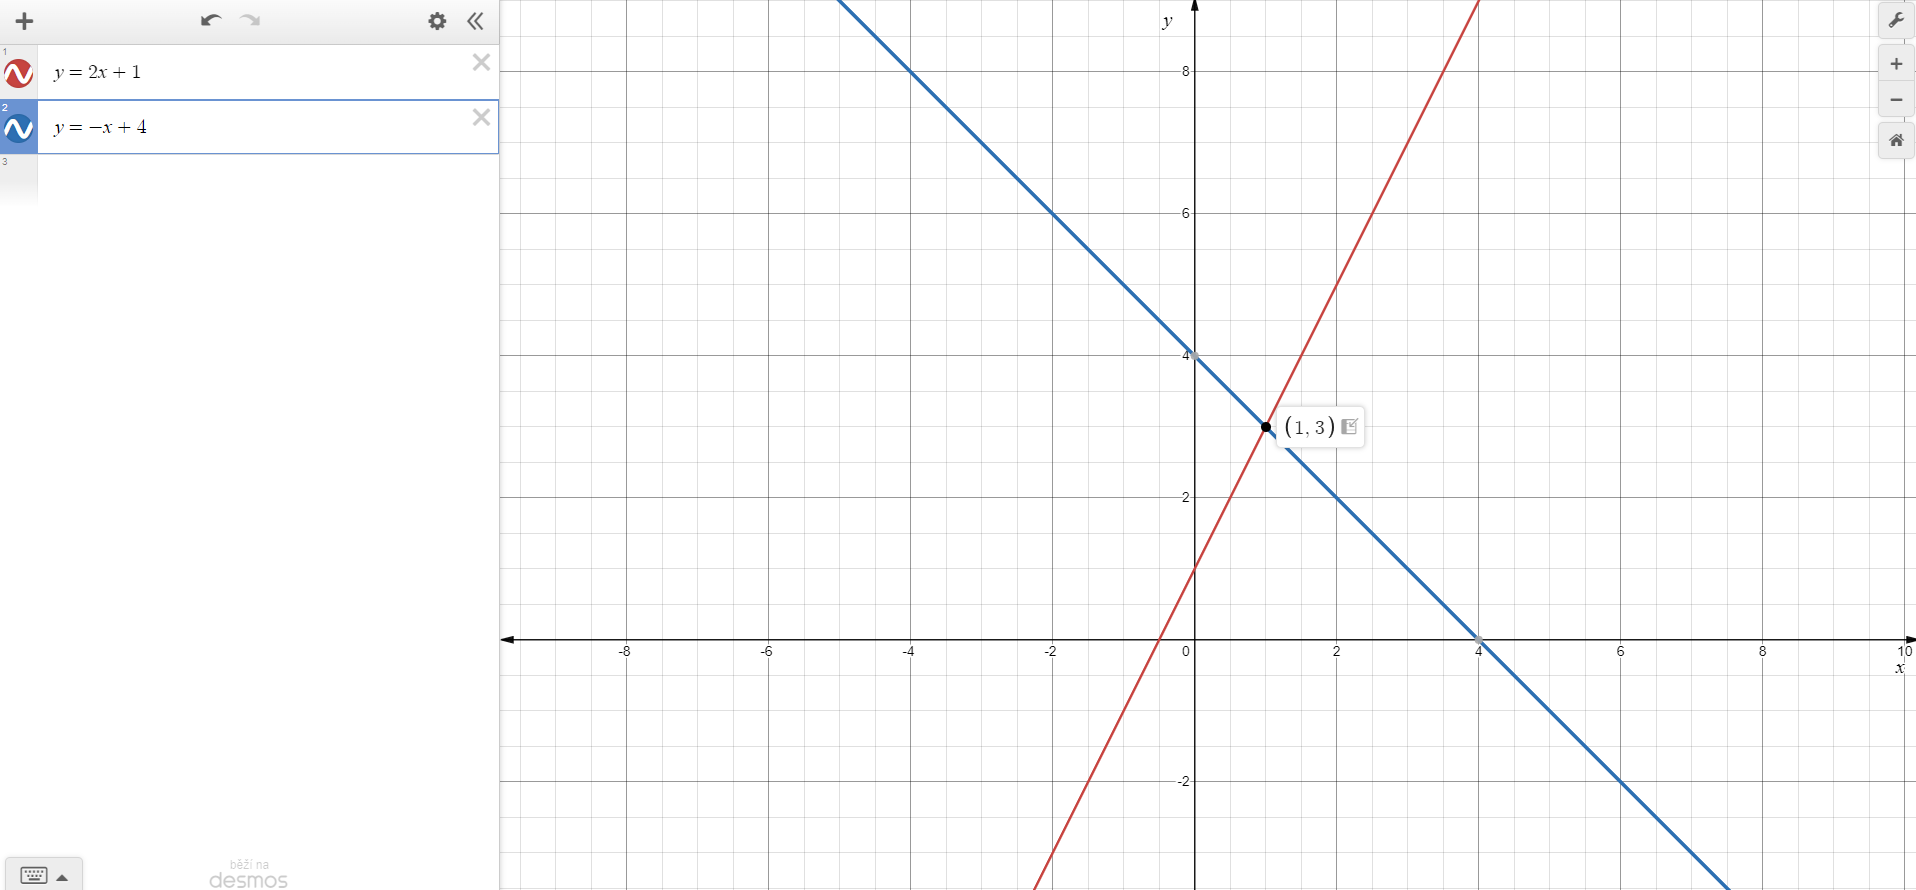
\includegraphics[width=0.5\linewidth]{img/4_soustava linearnich rovnic o dvou neznamych.png}
        \caption{$y=2x+1;y=-x+4$} 
        \label{fig:enter-label}
    \end{figure}
    
    \subsection{Počet řešení soustavy rovnic}
Nejsnazší zjištění počtu řešení je pře grafické řešení.\\
Pokud řešíme soustavu rovnic o \textbf{dvou neznámých} tak počet řešení odpovídá následujícím podmínkám:
 \begin{center}
            \begin{tabular}{||c| c|c||} 
             \hline
             \textbf{Situace} & \textbf{Geometrický význam} & \textbf{Počet řešení} \\ [0.5ex] 
             \hline\hline
             Přímky se protínají & Jediný průsečík & \textbf{Jedno řešení} \\
             \hline
             Přímky se překrývají & Jsou totožné & \textbf{Nekonečně mnoho řešení} \\
             \hline
             Přímky jsou rovnoběžné & Nikdy se neprotínají & \textbf{Žádné řešení}\\
             \hline
            \end{tabular}
            \end{center}
Ukázku můžete vidět v předešlém příkladu.\\\\
Pokud řešíme soustavu rovnic o \textbf{třech neznámých} tak počet řešení odpovídá následujícím podmínkám:
\begin{center}
            \begin{tabular}{||c| c|c||} 
             \hline
             \textbf{Situace} & \textbf{Geometrický význam} & \textbf{Počet řešení} \\ [0.5ex] 
             \hline\hline
             Tři roviny se protínají v jednom bodě & Společný průsečík všech & \textbf{Jedno řešení} \\
             \hline
             Tři roviny se protínají v přímce & Mají společnou přímku & \textbf{Nekonečně mnoho řešení} \\
             \hline
             Rovnoběžné nebo se neprotínají & Žádný společný bod & \textbf{Žádné řešení}\\
             \hline
            \end{tabular}
            \end{center}
\textbf{Příklad} tří rovin, které mají společný průsečík:
\begin{figure}[H]
        \centering
        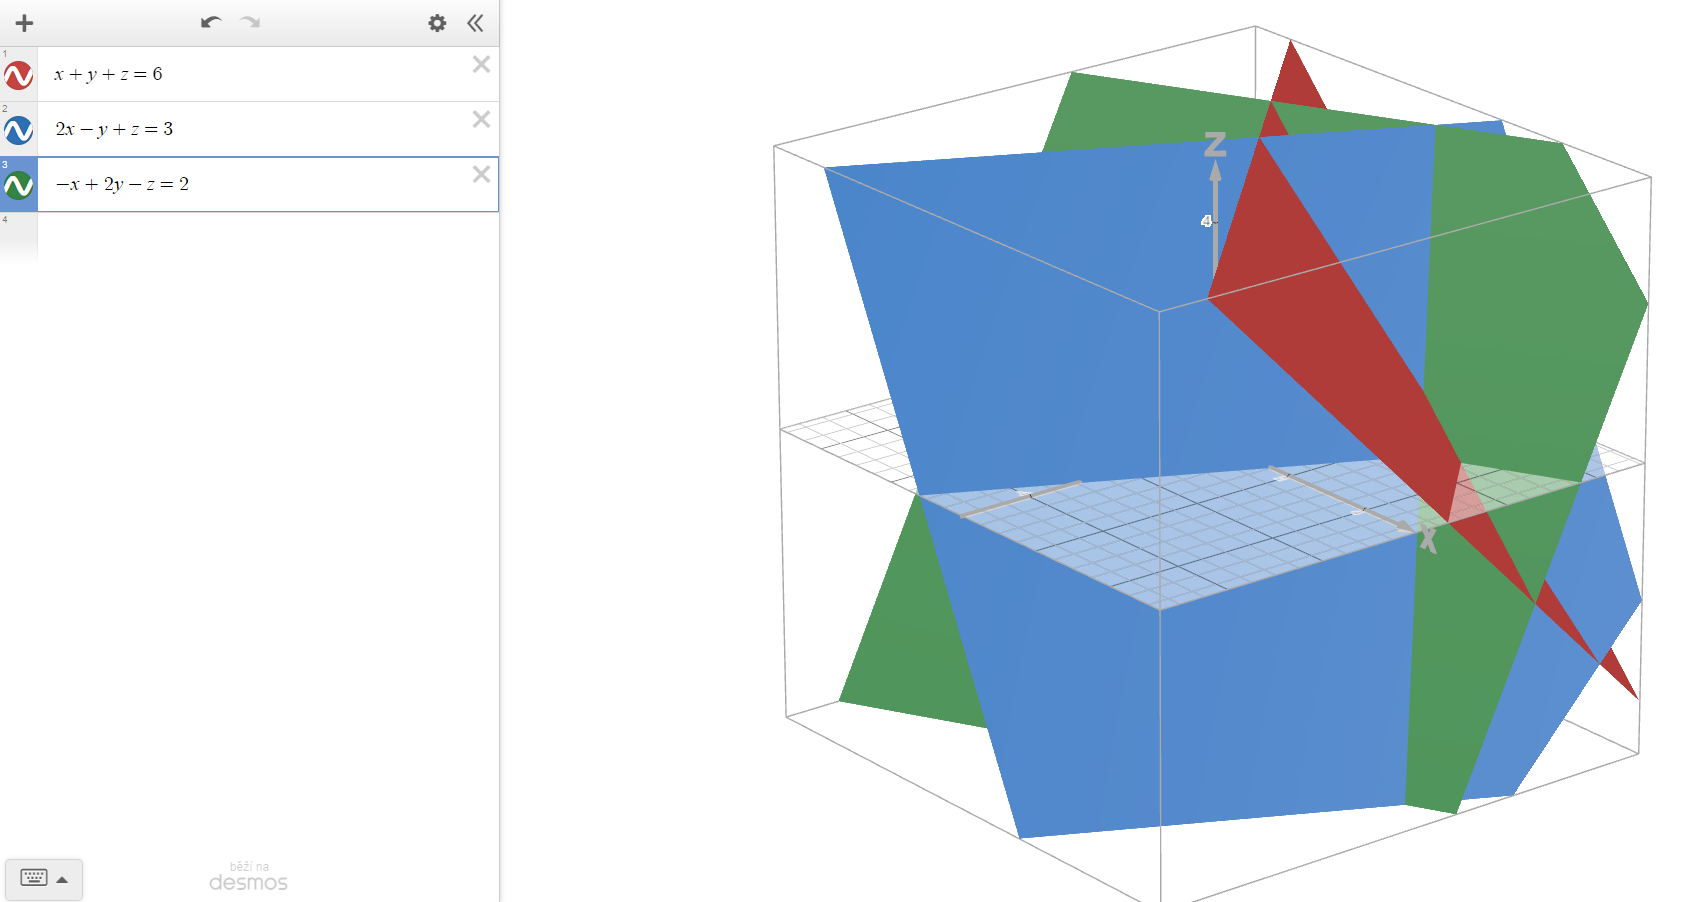
\includegraphics[width=0.5\linewidth]{img/4_soustava_rovnic_o_trech_neznamych.png}
        \caption{$y=6-x-z;y=2x+z-3;y=\frac{2+z+x}{2}$} 
        \label{fig:enter-label}
    \end{figure}